\documentclass[a4paper]{article}
%\usepackage{color}
\usepackage{listings}
\usepackage{multicol}
\usepackage{hyperref}
\usepackage{mathtools}
\usepackage{url}
\usepackage{pgfplots}
\usepackage{natbib}
\usepackage{xcolor}
\usepackage[english]{babel}
\usepackage[]{algorithm2e}
\usepackage{float}
\usepackage{hyperref}
%\usepackage[utf8]{inputenc}
\usepackage{amsmath}
\usepackage{natbib}
\usepackage{amsfonts}
\usepackage{graphicx}
\usepackage[colorinlistoftodos]{todonotes}
\usepackage[affil-it]{authblk}
\usepackage{tikz}
\usetikzlibrary{arrows}
\lstset {basicstyle=\tiny,
    language=C++,
    backgroundcolor=\color{blue!7},
    stringstyle=\color{red}}
\title{TER\\A new scattering based \\bioacoustic feature selector}
\author{Randall BALESTRIERO\\
\texttt{\url{randallbalestriero@gmail.com}}}
\affil{Department of Mathematics, Pierre et Marie Curie University Paris 6}
%\author{Vincent LOSTANLEN}
%\affil{Department of Computer Science, ENS Ulm}
%\author{Herv\'e GLOTIN}
%\affil{Aix Marseille Université, ENSAM, Marseille\\
%Universit\'e de Toulon, CNRS, LSIS UMR, La Garde\\
%Institut Universitaire de France (IUF), Paris
%}
%\author{St\'ephane MALLAT}
%\affil{Department of Computer Science, ENS Ulm}


\newcommand\norm[1]{\left\lVert#1\right\rVert}

\pdfminorversion=5 
\pdfcompresslevel=9 
\pdfobjcompresslevel=3

\date{}


\tikzset{
  treenode/.style = {align=center, inner sep=0pt, text centered,
    font=\sffamily},
  arn_n/.style = {treenode,   font=\sffamily\bfseries, draw=black,
     text width=1.5em},% arbre rouge noir, noeud noir
  arn_r/.style = {treenode, circle, red, draw=red, 
    text width=1.5em, very thick},% arbre rouge noir, noeud rouge
  arn_x/.style = {treenode, rectangle, draw=black,
    minimum width=0.5em, minimum height=0.5em}% arbre rouge noir, nil
}


\begin{document}

\maketitle
\section{Introduction}
With the scattering, new data representations are sparse and clean (more than spectrogram at least). We will use this to produce a robust and general bioacoustic feature extractor. The aim is to have a no tweaking technique working equally good on every species (even non birds). It has to be simple and fast to compute since it will be used on huge database.
\\
The advantage of this approach is a fast computation, robustness, good properties on the new representations as it will be explained later, and finally, no prior knowledge. The only assumptions are :
\begin{itemize}

\item (relatively) Sparse Scalograms (easiest feature extraction)
\item Given a frequency domain, the most present specie in it is the one of interest

\end{itemize} 
\section{Feature extractor}
This algorithm is based on two levels. The first one is simply a reconditioning of the scalogram in order to improve the second part performance : the feature extraction.
\\
I will present all the method and the examples are given in the end in order to improve the reader experience.
\subsection{Row Conditioning}
\subsubsection{Non biological sound suppression}
First we will remove background and non biological noises in the scalogram. In order to do this we will simply compute row median and row standard deviation. The ones with a higher median than the standard deviation are set to $0$. Meaning that if a line is too constant in time without any fluctuation then it is likely to be non biological.
\subsubsection{Row weighting}
The scalogram is not cleaner but still we are more interested in some frequency bands than others. In order to use this weighting into account, let's recompute the row standard deviation (or simply set to $0$ the coefficients corresponding to the lines we previously set to $0$). 
\\
After normalizing this vector (max set to $1$) we the scalogram by this vector.
The lines with high variations will be enhanced in contrast to the other ones.
\subsection{Word Extraction}
Now we have a real clean and sparse scalogram without any noise. We perform the word extraction. Note that we first perform word extraction and then compute song extraction which will be based on this part.
\\
The concept is really simple and is actually taken from finance with buying and selling signals. Let's take the column standard deviations (this gives us a long vector). Now we will treat it as a stock market price chart.\\
Thus, we will first take a long simple moving average (here on $1000$ coeffs). Then on this we compute an smaller exponential moving average (of half the previous size, so 500). We normalize the result and this will give the indicator line.
\\
Now we take the exponential moving average of this indicator line (of size $1000+500=1500$). This will be our signal line.
\\
The concept is simple, whenever the indicator line crosses its signal line by moving upward, this is a buy signal. When the indicator line crosses the signal line by moving downward, it is a sell signal.
\\
In order to avoid small noisy signals we also set an automatically selected minimum value for the signal line based on his histogram.
\\
This can be seen as modified Moving Average Convergence Divergence indicator. Where buying and selling signals are actually start and end point of the words.
\subsection{Song Extraction}
Now we have a word decomposition of the signal. In order to find out the position of the songs (which can be composed of multiple words) we will simply analyse the repartition of the words. Let's then look at the intervals (standard deviation) between the words. Given this we will look at each word and if they are closer than two times the standard deviation, we will concatenate them into a song. Note that a maximum step is set to $10000$ here so $1/4 s$ assuming than inside a song there should not be more than $1/4 s$ duration of silence.
\subsection{Examples}

\begin{figure}[H]
\begin{center}
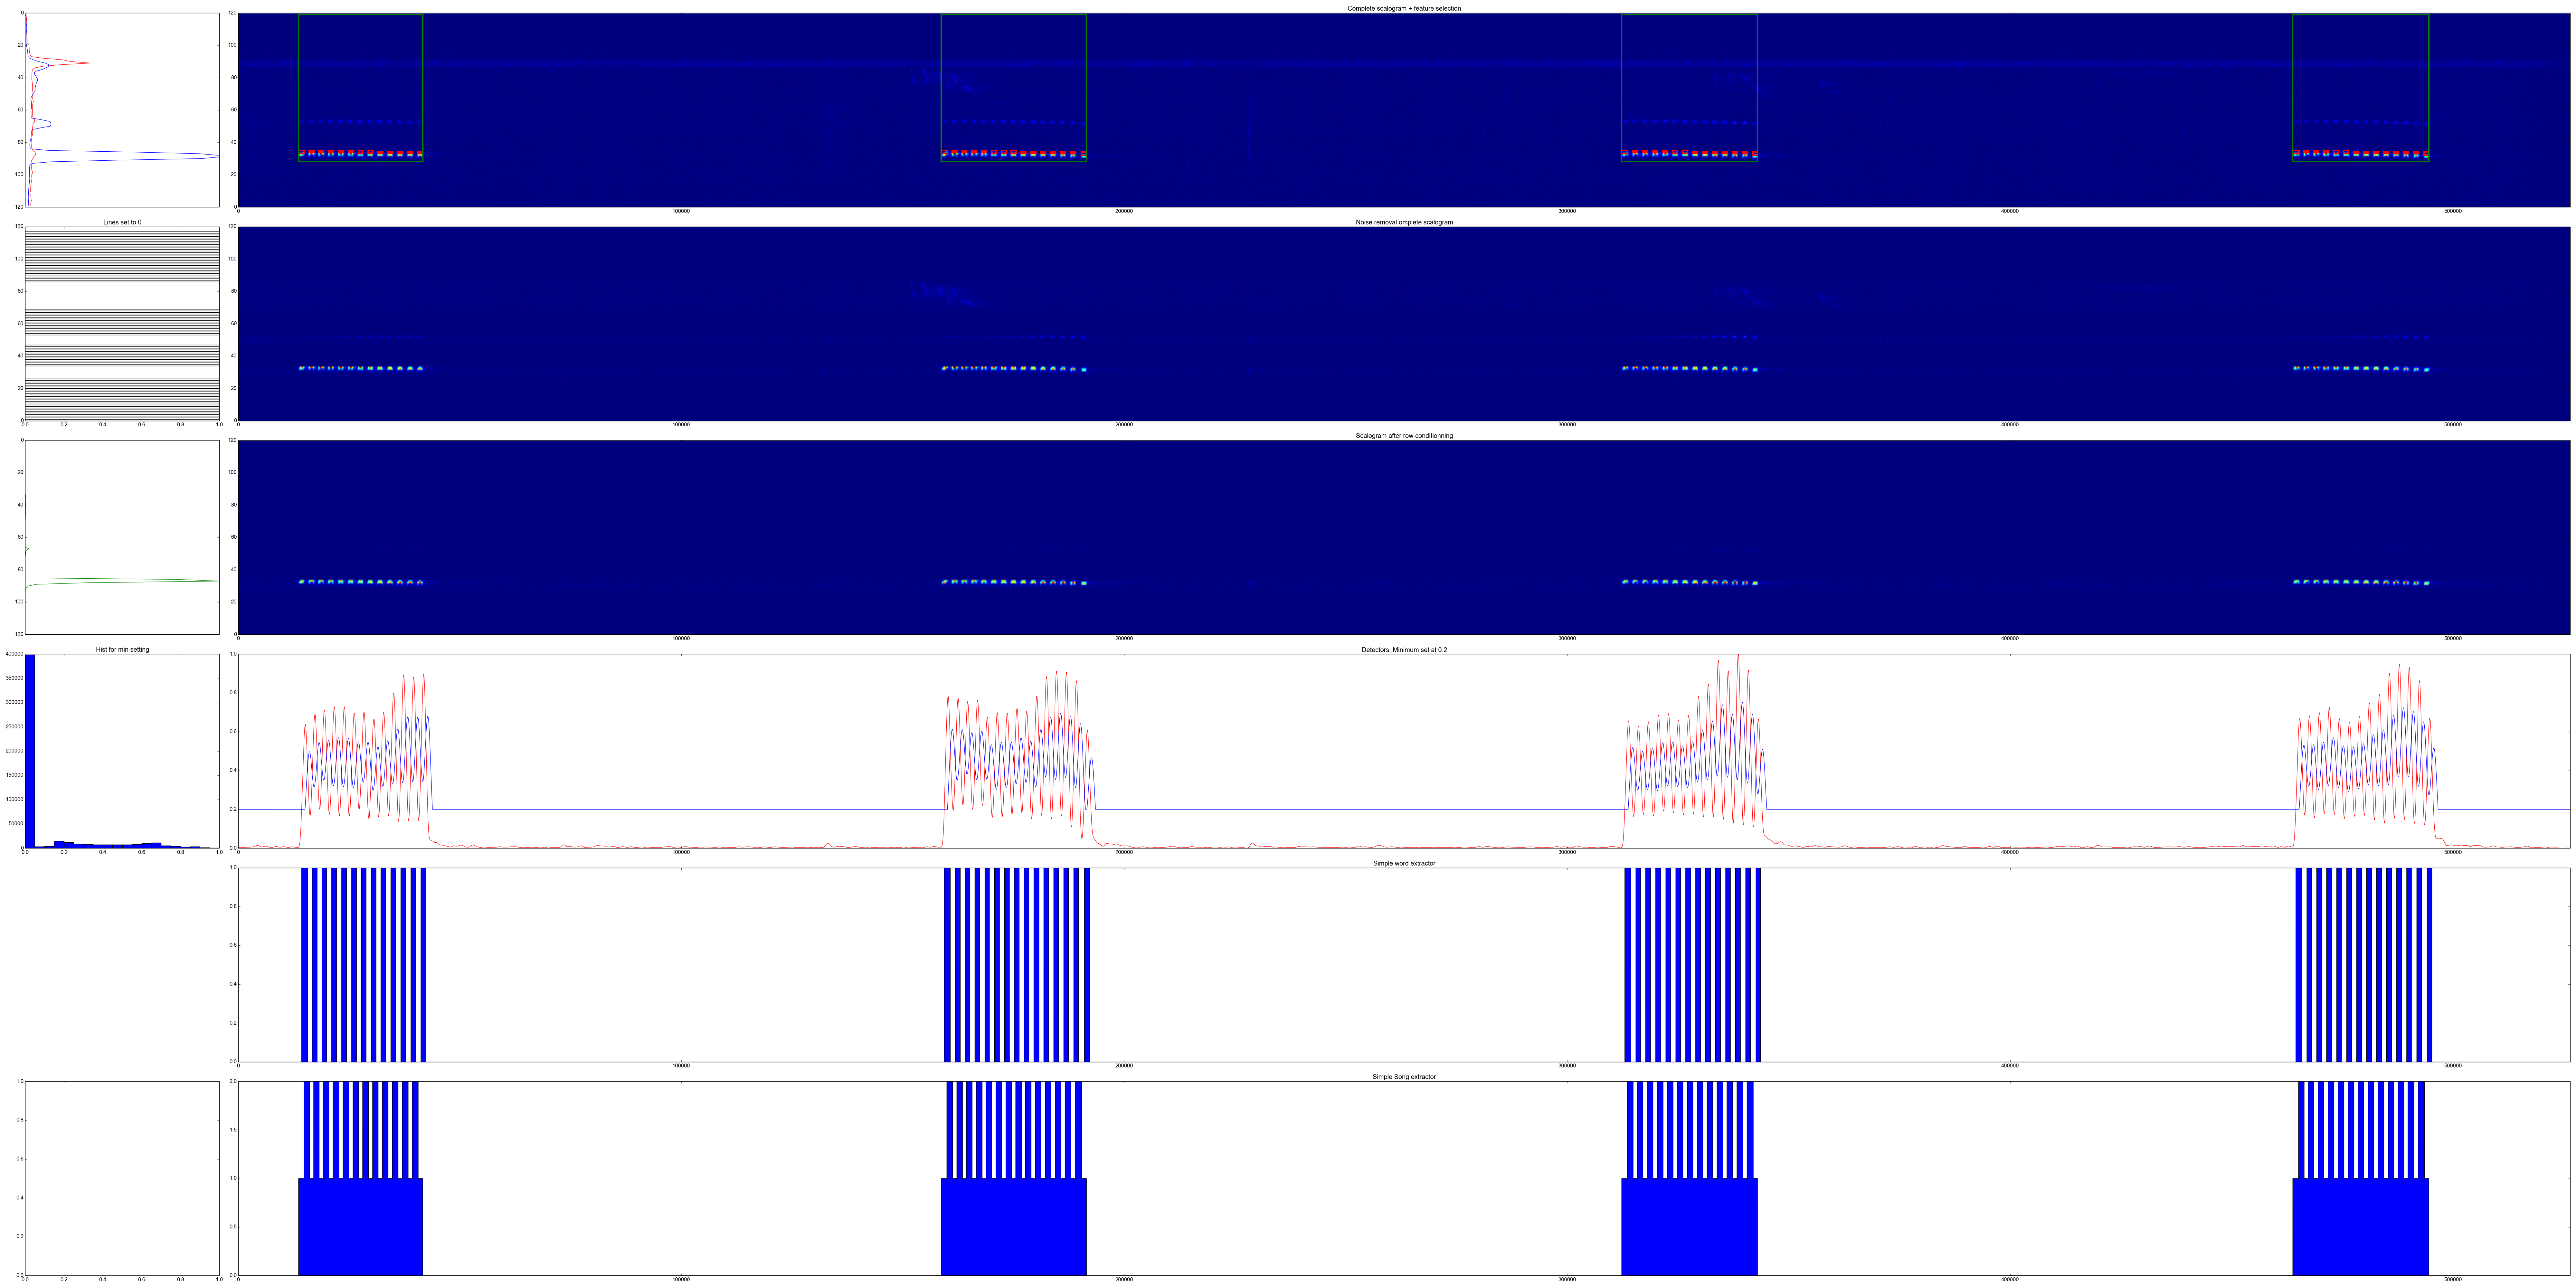
\includegraphics[scale=0.07]{1test.png}\caption{17 sec }
\end{center}
\end{figure}


\begin{figure}[H]
\begin{center}
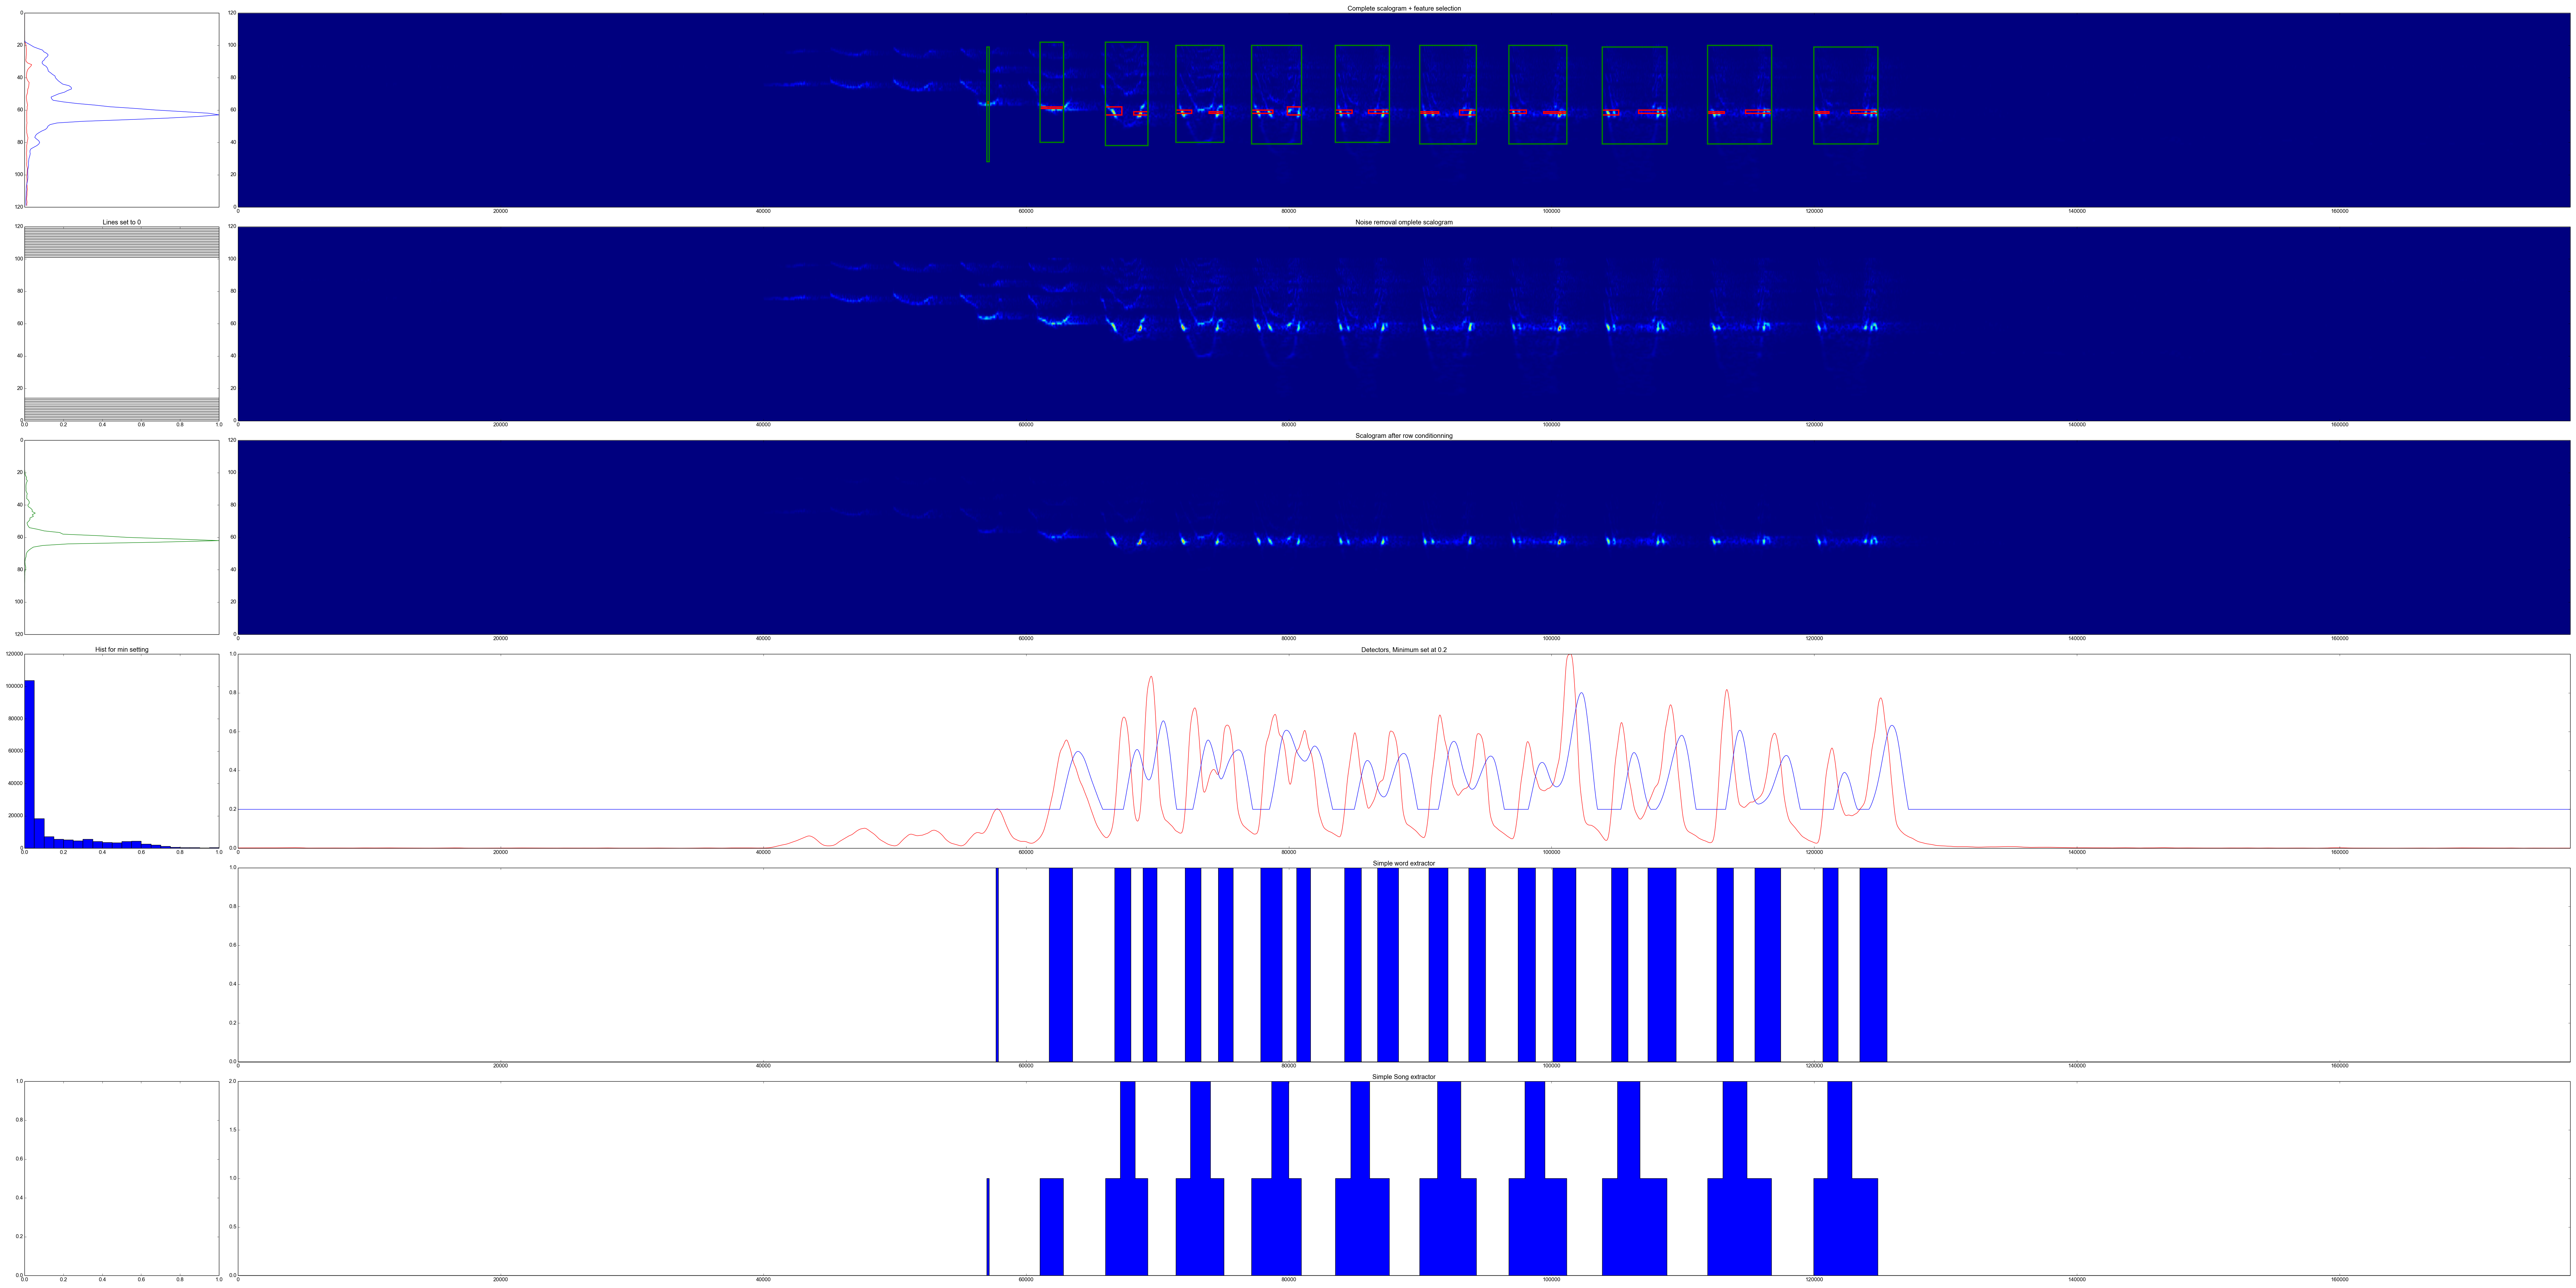
\includegraphics[scale=0.07]{2test.png}\caption{17 sec s}
\end{center}
\end{figure}


\begin{figure}[H]
\begin{center}
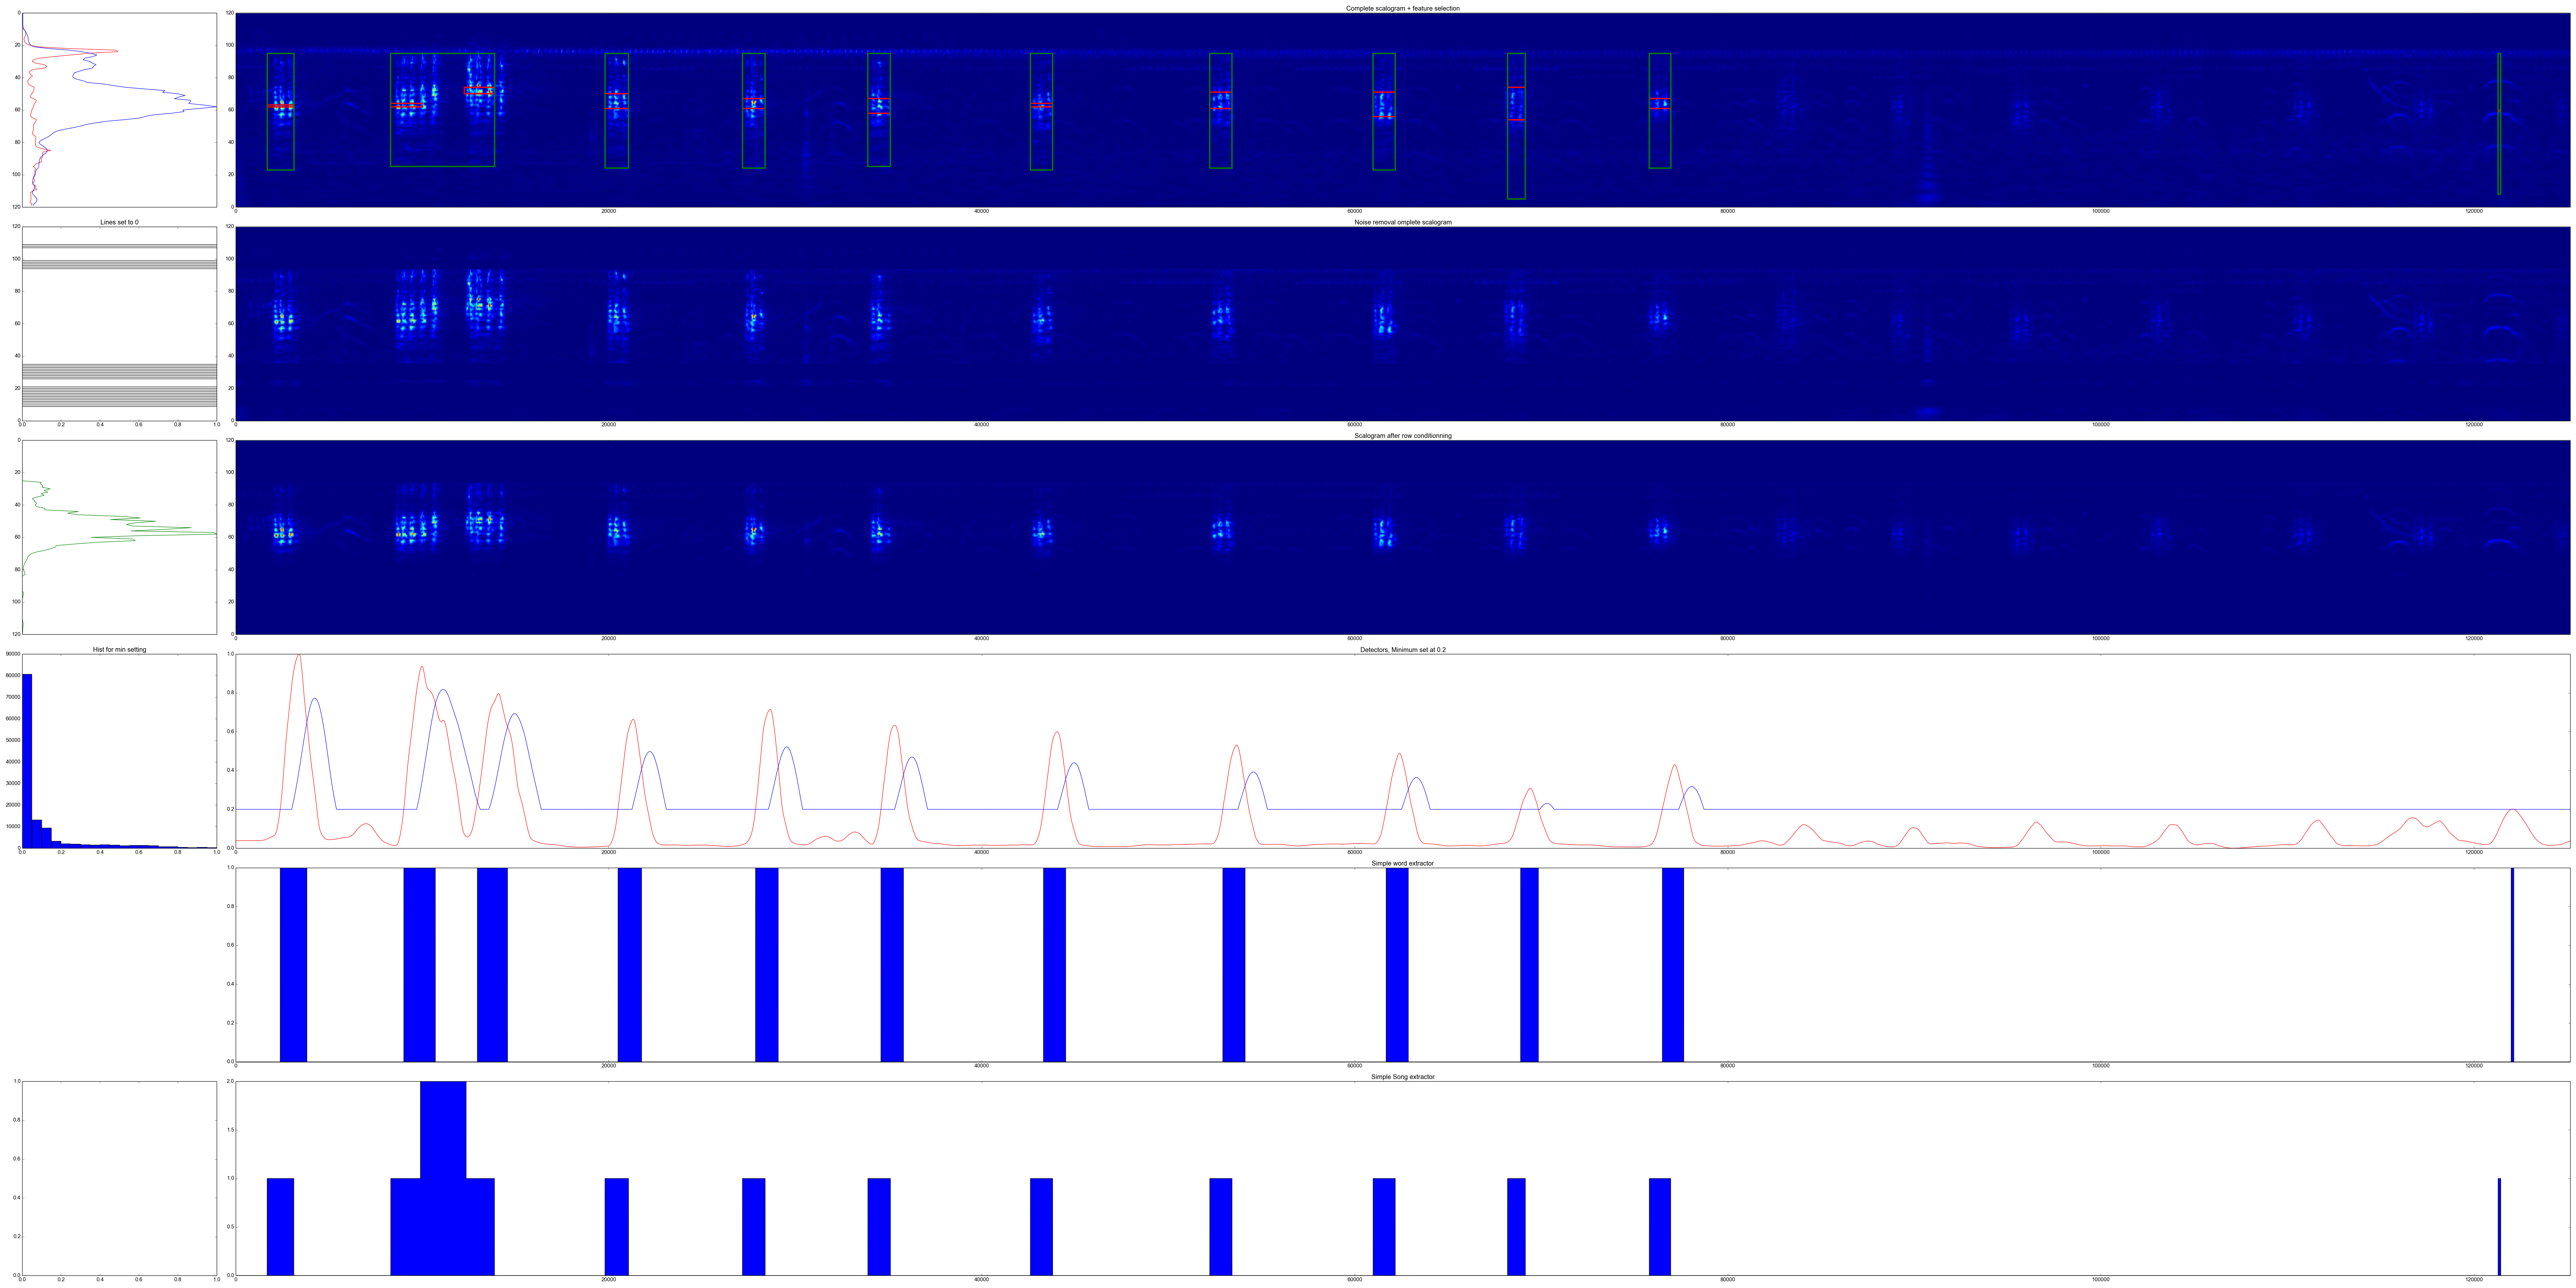
\includegraphics[scale=0.07]{3test.png}\caption{17 }
\end{center}
\end{figure}


\section{Application : BIRD TASK 2015 CHALLENGE}
TO DO cf .ppt
\section{Problem approach}
I want to use a new representation of the data (the scalogram) which then will be used for yet another new data representation in order to have a simple classification task afterwords. 
Then the process will be :
\begin{itemize}
\item Really fast but discriminative and robust algorithm to end with few possible species instead of the 1000. (typically 10)
\item A finer and more detailed classification process which will have to classify the signal between the (typically 10) possible species.
\end{itemize}

I will divide the description of this approach into two parts corresponding to the two main classification parts I will use for the task.
\\
The first one will be about building the new data  representation from the scalogram and how it is helping for the second part.
\\
The final classification process. 
\\
Here is the schema of the approach :
\begin{itemize}
\item Find the bird songs in the two scalo (step 0)
\item Compare their duration (step 1) and the songs organization in the signal (how many per duration time,...) (step 1*)
\item Compare their "texture", density as a whole (step 2)
\item Compare "words" composing the song as new individual features (step 3)
\end{itemize}
The part 1 will be step 1, 1* and 2 whereas part 2 will be the step 3. I consider step 0 as a preprocessing task which will be described as an independent part.
\subsection{Scalogram}
TO DO
Let's first describe briefly why I want to use scalogram as "raw input" for my algorithm.
Really sparse matrix, basically an improved spectrogram. Almost no computation cost.
\subsection{Bird Song characterization}

The main idea here is to keep the most discriminative information about a signal in order to quickly isolate candidates between a test example and the training set to work with for fine classification process.

My idea is to simply use what has been trained to perform this for thousands of year : the human approach.
If I ask anyone (other than ornithologists) to say if two signals belong to the same bird specie I assume the process will be close to :

Even though this can look as a decision tree it is actually not since we will allow little change in step 1 to be compensated in step 2 for example.

The goal is to characterize a signal by a small vector for the first classification step (step 1 + step 2). Typically : (song duration, song periodicity, texture information). This vector will us time in second for the first two components. This is interesting since we are invariant to translation (the length of the song is independent of the song position in the signal) and we are also invariant to "technical details". By this I mean even with signals from different sampling frequencies we will have the exact same components since to have the duration in second we use the sampling frequency. These two properties are I think really interesting for a first discrimination process. The texture component as yet to be define, a tuple (Mean, Variance) could be minimalist.
\\

\subsection{Illustration of this approach}
Let's compare three pairs of signals. We first consider \ref{figure1} and \ref{figure2}. We can see that the duration of the song is not really close plus given a time unit, the first one seems to have a slower ratio song$/$time unit. Of course in practice we will have statistics about the whole data set to quantify what is actually close or not for the song duration and all the other characteristics. The second pair is \ref{figure3} and \ref{figure4}. They seem to have a similar song duration and the number of song per time unit is not so far apart.
\\
Finally the last pair \ref{figure5} and \ref{figure6} is pretty easy to analyse. One can directly see the patterns are not at all of the same duration nor the same periodicity. So the third pair can already be ruled out just by these duration comparisons.
\begin{figure}[H]
\begin{center}
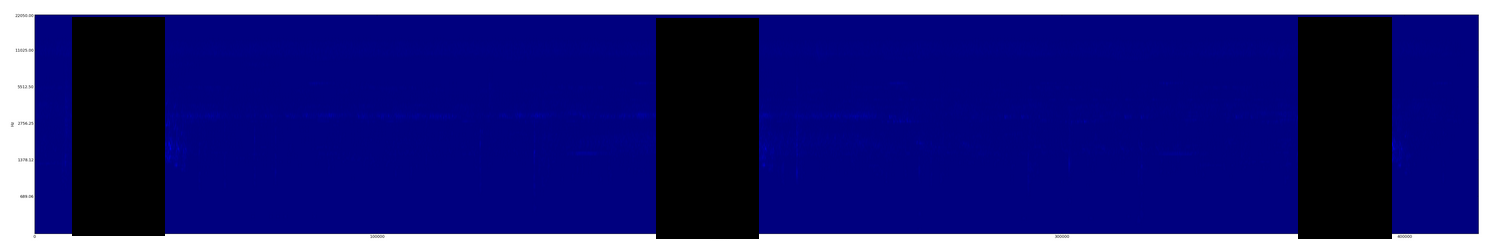
\includegraphics[scale=0.23]{XC91243_ter.png}\caption{17 sec signal, song duration : 1 sec, XC91243}\label{figure1}
\end{center}
\end{figure}


\begin{figure}[H]
\begin{center}
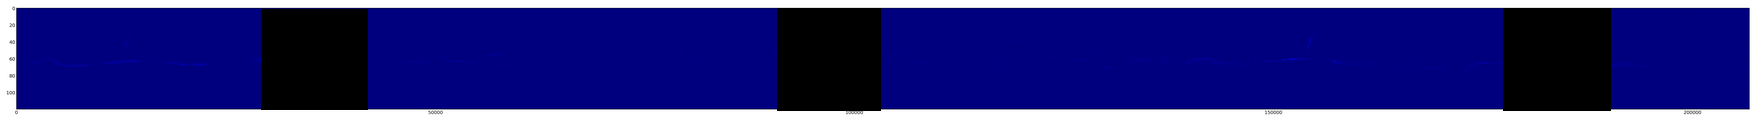
\includegraphics[scale=0.2]{XC81545_ter.png}\caption{9 sec signal, song duration : 0.7 sec, XC81545}\label{figure2}
\end{center}
\end{figure}


\begin{figure}[H]
\begin{center}
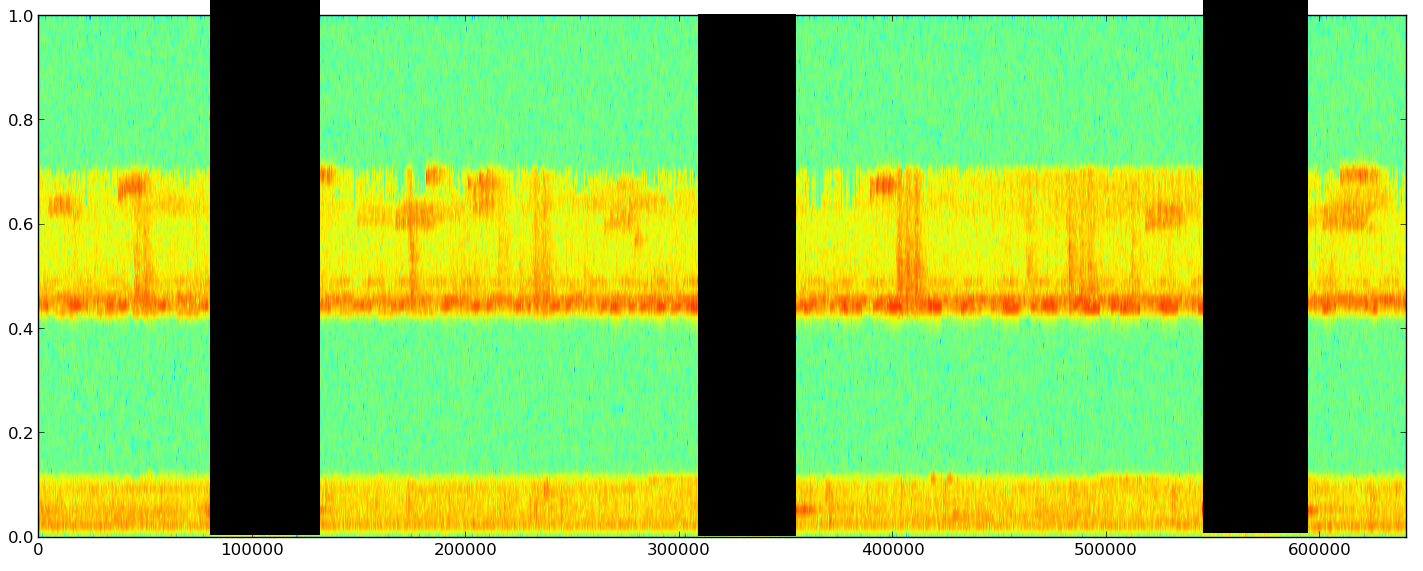
\includegraphics[scale=0.2]{RN11802.png}\caption{28 sec signal, song duration : 2 sec, RN11802}\label{figure3}
\end{center}
\end{figure}

\begin{figure}[H]
\begin{center}
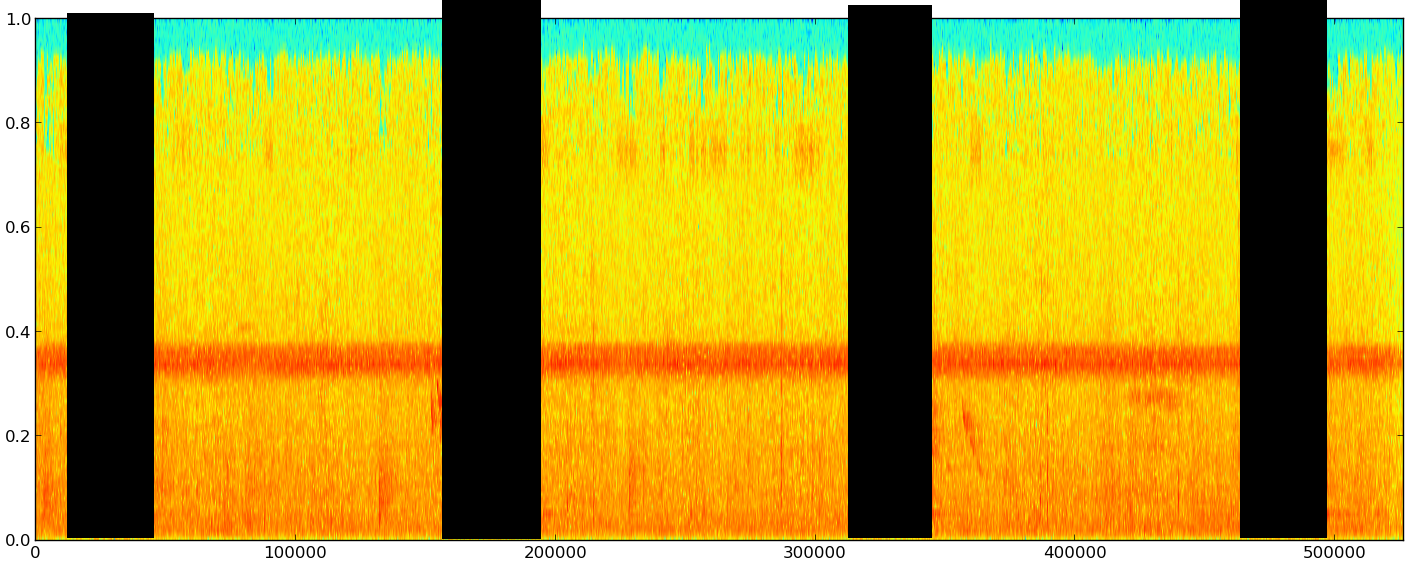
\includegraphics[scale=0.2]{RN2320.png}\caption{24 sec signal, song duration : 1.9 sec, RN2320}\label{figure4}
\end{center}
\end{figure}


\begin{figure}[H]
\begin{center}
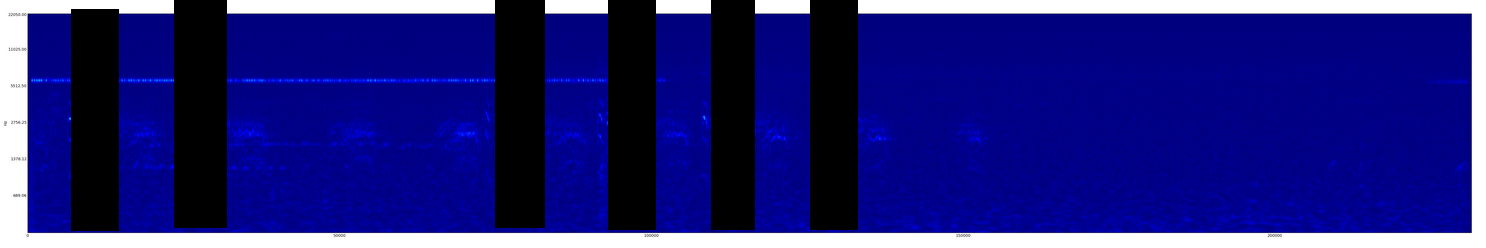
\includegraphics[scale=0.2]{XC9653.png}\caption{10 sec signal, song duration : 0.3 sec, XC9653}\label{figure5}
\end{center}
\end{figure}



\begin{figure}[H]
\begin{center}
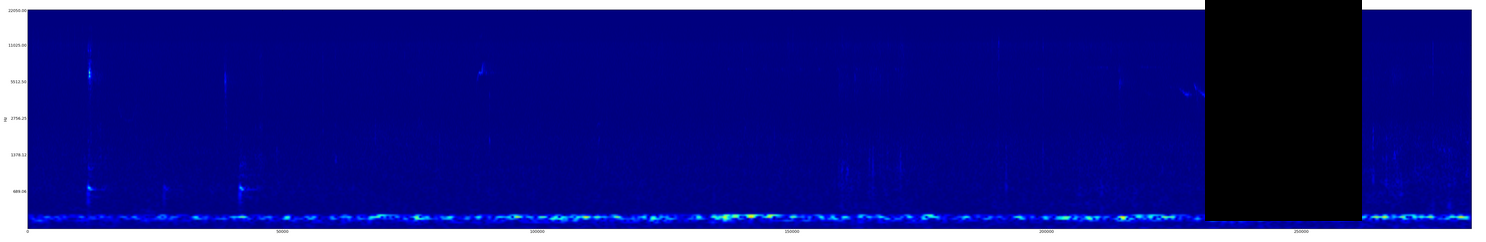
\includegraphics[scale=0.2]{XC93509.png}\caption{12 sec signal, song duration : 2 sec, XC93509}\label{figure6}
\end{center}
\end{figure}

So now let's look into the texture comparison for the first pair  \ref{figure7} and \ref{figure8}. Only considering the density and texture of the song it is not really easy to say that the song are different. So we can't rule out the same specie possibility yet.

Now about the second pair we have \ref{figure9} and \ref{figure10}. Now here the density is also pretty close. We can't judge yet of the specie relation.



Of course in these two example, the texture comparison wasn't useful but it will be when comparing the $1000 species$.
Now finally let's compare each word composing the songs.
In this final step we can clearly see that the first pair is not from the same specie while the second one is.

\begin{figure}[H]
\begin{center}
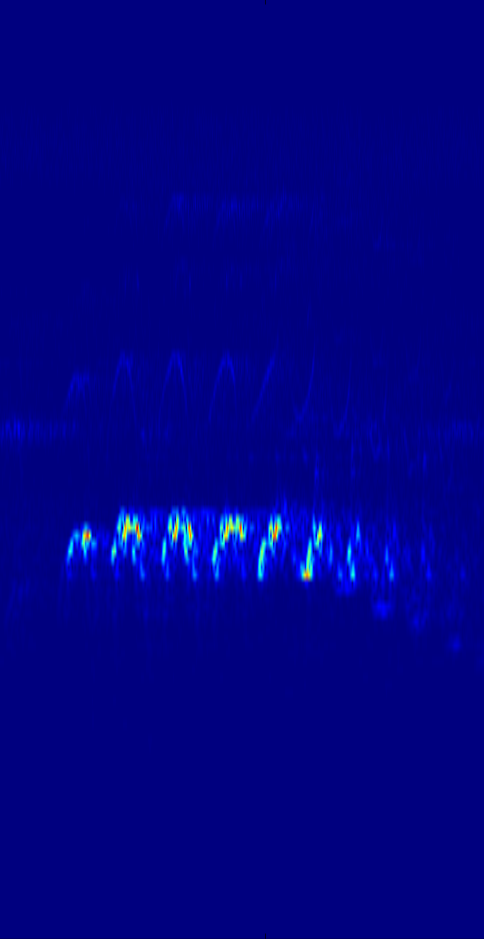
\includegraphics[scale=0.2]{XC91243_feature.png}\caption{XC91243}\label{figure7}
\end{center}
\end{figure}

\begin{figure}[H]
\begin{center}
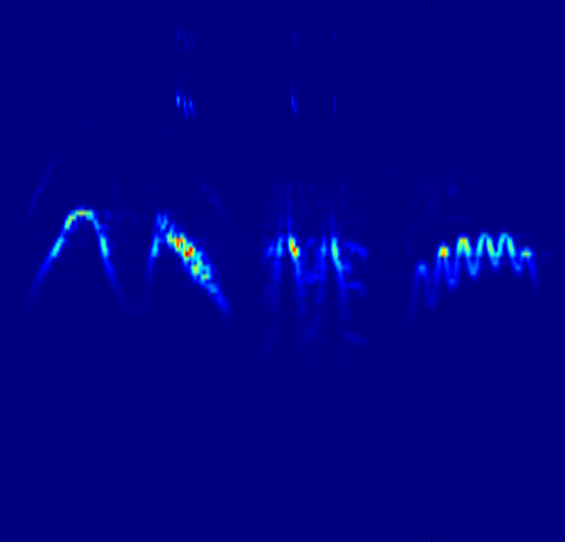
\includegraphics[scale=0.2]{XC81545_feature.png}\caption{XC81545}\label{figure8}
\end{center}
\end{figure}

\begin{figure}[H]
\begin{center}
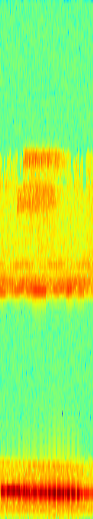
\includegraphics[scale=0.2]{RN11802_feature.png}
\caption{RN11802}\label{figure9}
\end{center}
\end{figure}

\begin{figure}[H]
\begin{center}
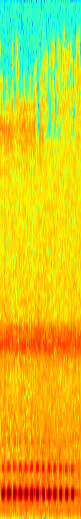
\includegraphics[scale=0.2]{RN2320_feature.png}\caption{RN2320}\label{figure10}
\end{center}
\end{figure}

\subsection{Classification process}
The classification process will be as follow.
For all the signal we have the small characterizing vector. We compute it for the test set example. We do a simple KNN in order to track the most likely candidates for more detailed comparisons. Let's say we keep the 10 signals closest to the one we aim to classify.
The next classification part is not yet well defined. For example,
now we end up with the following situation : given this signal I want to find the one out of 10 which are the closest. Of we could simply make a majority vote first, then compare more deeply (with the intra song features or "words") and so on.
\section{Song extraction}

wav names :



\end{document}
